This chapter establishes the technical and programmatic background on which
the remainder of the thesis builds. The problem introduced in
Chapter~\ref{ch:intro}, that a large, heterogeneous, and geographically
distributed inventory of \gls{UNF} must eventually be managed rather than only
stored, draws together several areas that have historically been developed
in isolation: the characteristics of the national inventory itself, the
simulation tools used to model fuel cycles, the transmutation technology
proposed to consume long-lived actinides, and the research program within
which this work is situated. Each is reviewed in turn.
Section~\ref{sec:unf} describes the scale, distribution, and composition of
\gls{UNF} in the United States and the assembly-level data that characterize
it. Section~\ref{sec:cyclus} introduces the \Cyclus agent-based fuel cycle
simulation framework and the modeling capabilities on which the archetypes
developed in this work depend. Section~\ref{sec:ads} presents
accelerator-driven systems and their role in minor actinide transmutation.
Section~\ref{sec:einstein} situates the thesis within the \gls{EINSTEIN}
project and the broader \gls{ARPAE} \gls{NEWTON} program.
Section~\ref{sec:litrev} reviews prior fuel cycle simulations of
transmutation systems, and Section~\ref{sec:gap} draws these threads together
to identify the specific research gap that this thesis addresses.


\section{Used Nuclear Fuel in the United States}
\label{sec:unf}

\gls{UNF}, also commonly called spent nuclear fuel, is nuclear
fuel that has been removed from a reactor because it can no longer efficiently
support the desired operating cycle. Although the fuel is no longer used in
the reactor, it remains thermally hot and highly radioactive because it
contains radioactive fission products, plutonium, and minor actinides produced
during irradiation \cite{nrc_high_level_waste}. The term ``used'' is
particularly appropriate because the discharged material is not completely
depleted: most of its uranium remains, and the fuel also contains newly
generated fissile isotopes that could potentially be recovered and reused.

The radioactivity and heat generation of \gls{UNF} decrease with time, but they do
so over multiple timescales. Short-lived fission products dominate the
radiation field and decay heat immediately following discharge. At longer
times, plutonium and the minor actinides become increasingly important because
many of these isotopes have half-lives ranging from hundreds to tens of
thousands of years. Consequently, untreated commercial \gls{UNF} may require
isolation over timescales on the order of \(10^{5}\) years before its
radiotoxicity approaches that of the natural uranium ore from which the fuel
was originally produced \cite{arpa_e_newton_2025}. The long duration of this
hazard is a central challenge in nuclear waste management.

The internationally accepted approach for the permanent isolation of \gls{UNF} and
high-level radioactive waste is disposal in a deep geologic repository
\cite{doe_waste_strategy_2013}. The United States, however, does not currently
operate a permanent repository for commercial \gls{UNF}. Until such a repository or
another disposition pathway becomes available, reactor licensees must store
the fuel at or near the sites where it was generated
\cite{nrc_high_level_waste,nrc_spent_fuel_storage}. Newly discharged fuel is
first placed in water filled spent fuel pools, which provide both cooling and
radiation shielding. After several years of cooling, assemblies may be
transferred to sealed dry storage systems at independent spent fuel storage
installations.

Because a national disposal system has not yet been implemented\cite{nrc_spent_fuel_storage}, the
geographic distribution of \gls{UNF} largely reflects the historical deployment of
the U.S. reactor fleet. Most commercial fuel remains at operating or
decommissioned nuclear power plant sites, including locations at which the
reactor itself has been permanently shut down. The result is a distributed
inventory that must eventually be transported, consolidated, processed, or
disposed of\cite{carter_banerjee_inventory_2024}.

Approximately \(99{,}000\) \gls{MTU} from commercial
pressurized water reactors and boiling water reactors
had been permanently discharged in the United States. This inventory grows by
roughly 2,000 \gls{MTU} per year as operating reactors discharge fuel \cite{GC-859},
and the current reactor fleet is projected to have generated about 140,000 \gls{MTU}
in total by 2060. The U.S. \gls{DOE} managed an additional inventory
of approximately \(2{,}446\) \gls{MTHM}, excluding most naval fuel.
Unlike the comparatively standardized commercial light water reactor
inventory, \gls{DOE}-managed \gls{UNF} includes fuel from defense production reactors,
research and test reactors, early demonstration reactors, and other specialized
programs. Altogether, \gls{UNF} and primary reprocessing wastes were distributed
across more than 100 locations in 39 states
\cite{carter_banerjee_inventory_2024}.

Table~\ref{tab:us-unf-summary}, compiled from the PNNL \emph{Spent Nuclear
Fuel and Reprocessing Waste Inventory} report
\cite{carter_banerjee_inventory_2024} and the GC-859 Nuclear Fuel Data Survey
\cite{GC-859}, summarizes the scale and distribution of this inventory.
Commercial fuel dominates the national inventory by mass, while
\gls{DOE}-managed material is considerably more diverse in enrichment, fuel
form, cladding, geometry, and irradiation history.


\begin{table}[htbp]
    \centering
    \caption{The U.S. inventory of used nuclear fuel and primary
    reprocessing waste was distributed among commercial, \gls{DOE}, research, and
    legacy waste sites. Data from
    \cite{carter_banerjee_inventory_2024,GC-859}.}
    \label{tab:us-unf-summary}

    \begin{threeparttable}
    \begin{tabularx}{\textwidth}{@{}Xr@{}}
        \toprule
        \textbf{Inventory category} & \textbf{Reported quantity} \\
        \midrule
        Commercial \gls{UNF} at nuclear power plant and \gls{ISFSI} sites
            & \(90{,}963\) \gls{MTHM} \\

        Permanently discharged \gls{PWR} fuel
            & \(135{,}645\) assemblies; \(59{,}013\) \gls{MTHM} \\

        Permanently discharged \gls{BWR} fuel
            & \(179{,}466\) assemblies; \(32{,}023\) \gls{MTHM} \\

        Commercial dry storage canisters or casks
            & \(3{,}862\) \\

        \gls{DOE}-managed \gls{UNF}
            & approximately \(2{,}446\) \gls{MTHM}\tnote{a} \\

        \gls{UNF} at university, government, and commercial research sites
            & approximately \(1\) \gls{MTHM} \\

        Commercial nuclear power plant and \gls{ISFSI} sites storing \gls{UNF}
            & \(73\) sites \\

        Sites with all nuclear power reactors permanently shut down
            & \(20\) sites \\

        Operating commercial nuclear power reactors
            & \(94\) reactors \\

        Permanently shut down commercial nuclear power reactors
            & \(27\) reactors \\

        \gls{DOE} sites with \gls{UNF} storage or research reactors
            & \(6\) sites \\

        University research reactor sites
            & \(20\) sites \\

        Other government research reactor sites
            & \(4\) sites \\

        Commercial research and development sites with \gls{UNF}
            & \(4\) sites \\

        Primary reprocessing waste or high level waste sites
            & \(4\) sites \\
        \bottomrule
    \end{tabularx}

    \begin{tablenotes}[flushleft]
        \footnotesize
        \item[a] The detailed \gls{DOE} inventory total depends on the treatment
        of naval fuel and commercial fuel transferred to \gls{DOE} custody.
        The value shown here follows the inventory basis used in this work.
        Quantities are rounded and may therefore differ slightly among
        inventory summaries.
    \end{tablenotes}
    \end{threeparttable}
\end{table}

The commercial inventory has also changed in composition over the history of
the U.S. nuclear power program. In the early decades of light water reactor
operation, discharged fuel commonly had burnups below
\(20~\mathrm{GWd/\gls{MTU}}\), and initial enrichments were often near
\(2~\mathrm{wt}\%\) \ce{^{235}U}. Improvements in fuel design, reactor
operation, and fuel management strategies allowed utilities to extend cycle
lengths and extract more energy from each assembly. By the twenty-first
century, average discharge burnup had increased to approximately
\(50~\mathrm{GWd/\gls{MTU}}\), while typical initial enrichment approached
\(4.5~\mathrm{wt}\%\) \ce{^{235}U}
\cite{carter_banerjee_inventory_2024}.

Figure~\ref{fig:annual-burnup-enrichment} shows the increase in annual average
burnup and initial enrichment for U.S. light water reactor discharges between
1968 and 2022. Although pressurized water reactor and boiling water reactor
fuel follow somewhat different histories, both exhibit the same broad trend
toward higher enrichment and higher discharge burnup.

\begin{figure}[htbp]
    \centering
    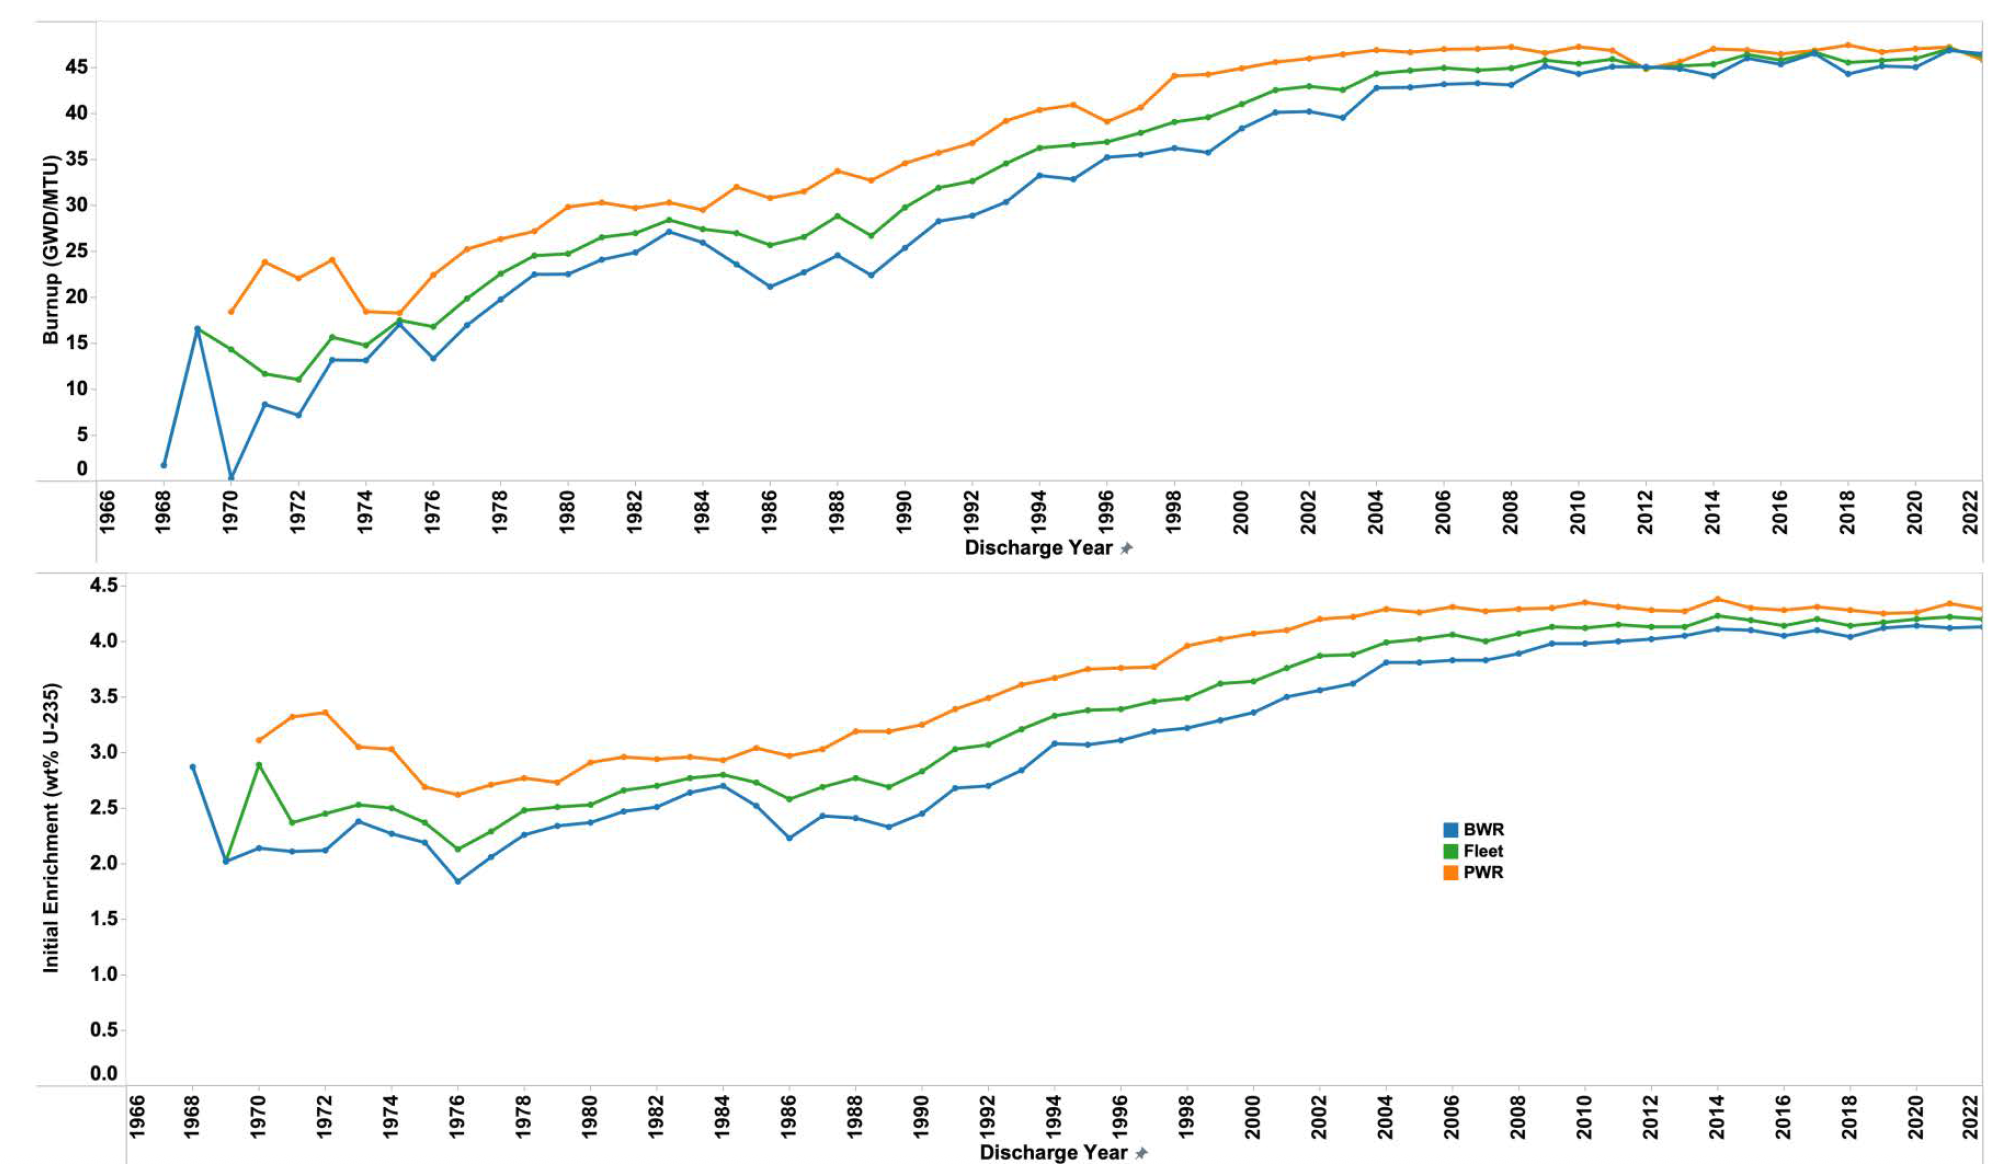
\includegraphics[width=\textwidth]
        {figures/burnup_enrichment.png}
    \caption{The annual average discharge burnup and initial
    \ce{^{235}U} enrichment of U.S. light water reactor fuel increased
    substantially between 1968 and 2022. Figure reproduced from \cite{carter_banerjee_inventory_2024}.}
    \label{fig:annual-burnup-enrichment}
\end{figure}


Figure~\ref{fig:assembly-burnup-enrichment} provides the corresponding
joint distribution of assembly burnup and initial enrichment in the inventory,
showing both the central concentration of the data and the smaller number of
assemblies at the extremes of the operating range.

\begin{figure}[htbp]
    \centering
    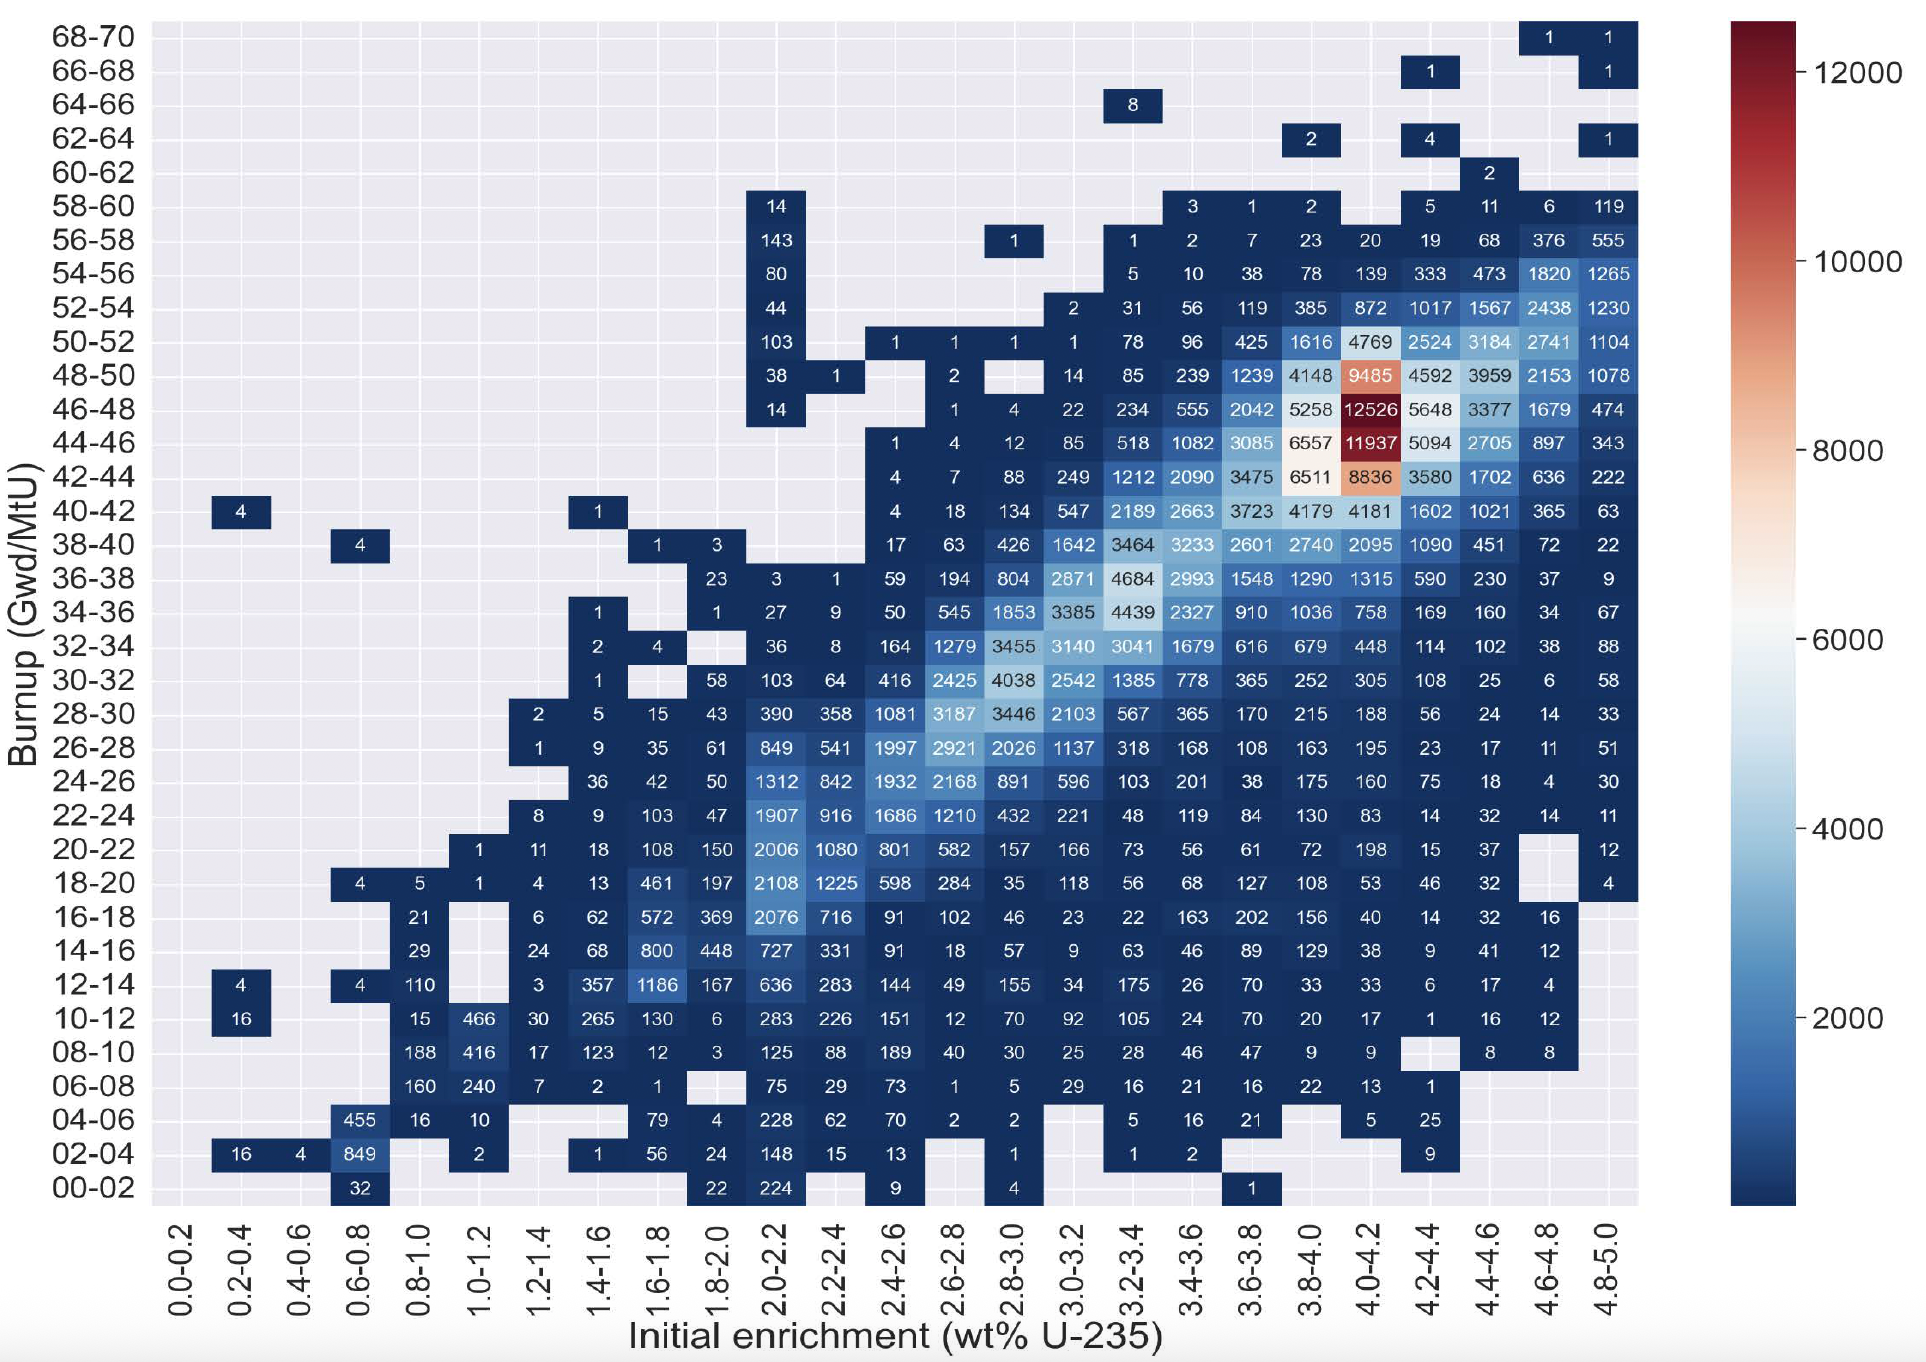
\includegraphics[width=\textwidth]{figures/assemblies.png}
    \caption{Burnup (GWd/MTHM) and initial enrichment (\% $^{235}U$)
    distributions for spent nuclear fuel assemblies in the \glspl{LWR}
    inventory through December 2022. Figure reproduced from
    \cite{carter_banerjee_inventory_2024}.}
    \label{fig:assembly-burnup-enrichment}
\end{figure}

Higher burnup changes the isotopic composition of discharged fuel. During
irradiation, neutron capture in \ce{^{238}U} produces plutonium isotopes, while
successive neutron capture and decay reactions generate neptunium, americium,
and curium. Extending irradiation therefore generally increases the production
of plutonium and minor actinides within an assembly, although the exact
inventory depends on enrichment, reactor type, neutron spectrum, power
history, and cooling time. The modern \gls{UNF} inventory is consequently not
uniform: assemblies discharged in different decades contain different
quantities of fissile material, transuranic elements, fission products, and
decay heat\cite{carter_banerjee_inventory_2024}.

These compositional differences are important because the nuclides that
control \gls{UNF} behavior change with cooling time. Shortly after discharge,
fission products dominate decay heat. In particular, \ce{^{137}Cs} and
\ce{^{90}Sr}, together with their decay products, are major contributors over
the first several decades. Their heat output decreases substantially as they
decay. Over longer periods, transuranic isotopes, especially plutonium and
americium isotopes, become the dominant contributors to the remaining heat
and radiotoxicity
\cite{carter_banerjee_inventory_2024}.

This transition is significant for the U.S. waste management strategy. Storage can
allow short-lived fission products to decay, but short-term storage does not eliminate
the fundamental long-term burden posed by plutonium and the minor actinides.
In a once-through fuel cycle, these nuclides must otherwise remain isolated while they decay over much
longer timescales. Alternatively, actinides can be separated and irradiated in a
suitable neutron spectrum, where fission converts them into shorter-lived
fission products while releasing additional energy. Long-lived fission
products may also be candidates for specialized transmutation, but the
actinides are the principal component of \gls{UNF} that can be destroyed through
fission rather than managed solely by long-term storage and geologic
isolation\cite{iaea_ma_fuels_2009}.

The increasing mass, geographic dispersion, and transuranic content of the
U.S. \gls{UNF} inventory therefore motivate the fuel cycle simulations in this
work. A realistic assessment of accelerator-driven transmutation must
represent not only the total mass of available fuel, but also the differences
among assemblies in discharge date, burnup, enrichment, location, and
isotopic composition. These attributes determine which portions of the
inventory can be selected, separated, and supplied to an accelerator-driven
system.

%%%%%%%%%%%%%%%%%%%%%%%%%%%%%%%%%%%%%%%%%%%%%%%%%%%%%%%%%%%%%%%%%%%%%%%%%%%%%%%%%%%%%%%%%%%%%%%%%%%%%%%%%%%%%%%%%%%%%%%%%%%%%%%%%%
%%%%%%%%%%%%%%%%%%%%%%%%%%%%%%%%%%%%%%%%%%%%%%%%%%%%%%%%%%%%%%%%%%%%%%%%%%%%%%%%%%%%%%%%%%%%%%%%%%%%%%%%%%%%%%%%%%%%%%%%%%%%%%%%%%%
%%%%%%%%%%%%%%%%%%%%%%%%%%%%%%%%%%%%%%%%%%%%%%%%%%%%%%%%%%%%%%%%%%%%%%%%%%%%%%%%%%%%%%%%%%%%%%%%%%%%%%%%%%%%%%%%%%%%%%%%%%%%%%%%
\section{The Cyclus Fuel Cycle Simulation Framework}
\label{sec:cyclus}

The two archetypes developed in this thesis are implemented within \Cyclus,
and their behavior can only be understood in relation to the framework's
underlying model of facilities, materials, and exchange. This section reviews
the aspects of \Cyclus most relevant to that implementation and introduces the agent-based
structure of the framework and how it represents fuel cycle facilities and
their interactions over time. Then moving on to describe how materials and their
isotopic compositions are represented and how radioactive decay is applied,
which is central to tracking the evolving minor actinide vector on which this
work depends and explains the \gls{DRE}, the mechanism through
which facilities request, offer, and trade resources at each time step.

\subsection{Framework Basics}
\label{subsec:cyclus-framework-basics}

\Cyclus is an open-source, agent-based nuclear fuel cycle simulation
framework designed to represent the deployment, operation, and interaction
of nuclear fuel cycle facilities over time. The framework tracks discrete
facilities and material resources rather than representing the fuel cycle
solely through aggregated fleet-level flows. This design supports analyses
in which individual facility behavior, material availability, and institutional
decisions influence system level outcomes
\cite{huff_fundamental_2016}.

Agents in a \Cyclus simulation are organized into three hierarchical types:
regions, institutions, and facilities. Regions form the highest organizational
level and may represent countries, geographic areas, or other broad
groupings. Institutions operate within regions and manage the deployment
and retirement of facilities. Facilities represent physical or functional
components of the nuclear fuel cycle, including mines, enrichment plants,
reactors, separations facilities, storage facilities, and repositories
\cite{huff_fundamental_2016}.

A \Cyclus simulation advances through discrete time steps, commonly
defined as months. During each time step, facilities may request resources,
offer available resources, conduct material transactions, process their
inventories, and update their internal states. Modeling facilities and time
discretely allows the framework to capture effects such as asynchronous
reactor refueling, temporary shortages of fuel cycle materials, and 
differences in facility deployment and retirement schedules\cite{gidden_agent-based_2015}.

The behavior of each agent is defined by an \emph{archetype}. Archetypes
are modular software components that implement the physical behavior,
operating logic, or decision rules of a region, institution, or facility.
They are compiled independently from the \Cyclus kernel and loaded
dynamically at the beginning of a simulation. This plug in architecture
allows alternative models of the same fuel cycle process to be exchanged
without modifying the core simulation framework
\cite{huff_fundamental_2016,scopatz_cyclus_2015}.

The \Cyclus kernel provides shared simulation services, including time
management, agent deployment, resource tracking, data recording, and
resource exchange. Archetypes access these services through the agent
application programming interface. As illustrated in
Figure~\ref{fig:cyclus-architecture}, the kernel provides the central
simulation environment, the agent interface connects the kernel to agent
models, and independently developed archetype libraries provide the
behavior of the simulated regions, institutions, and facilities.

\begin{figure}[htbp]
    \centering
    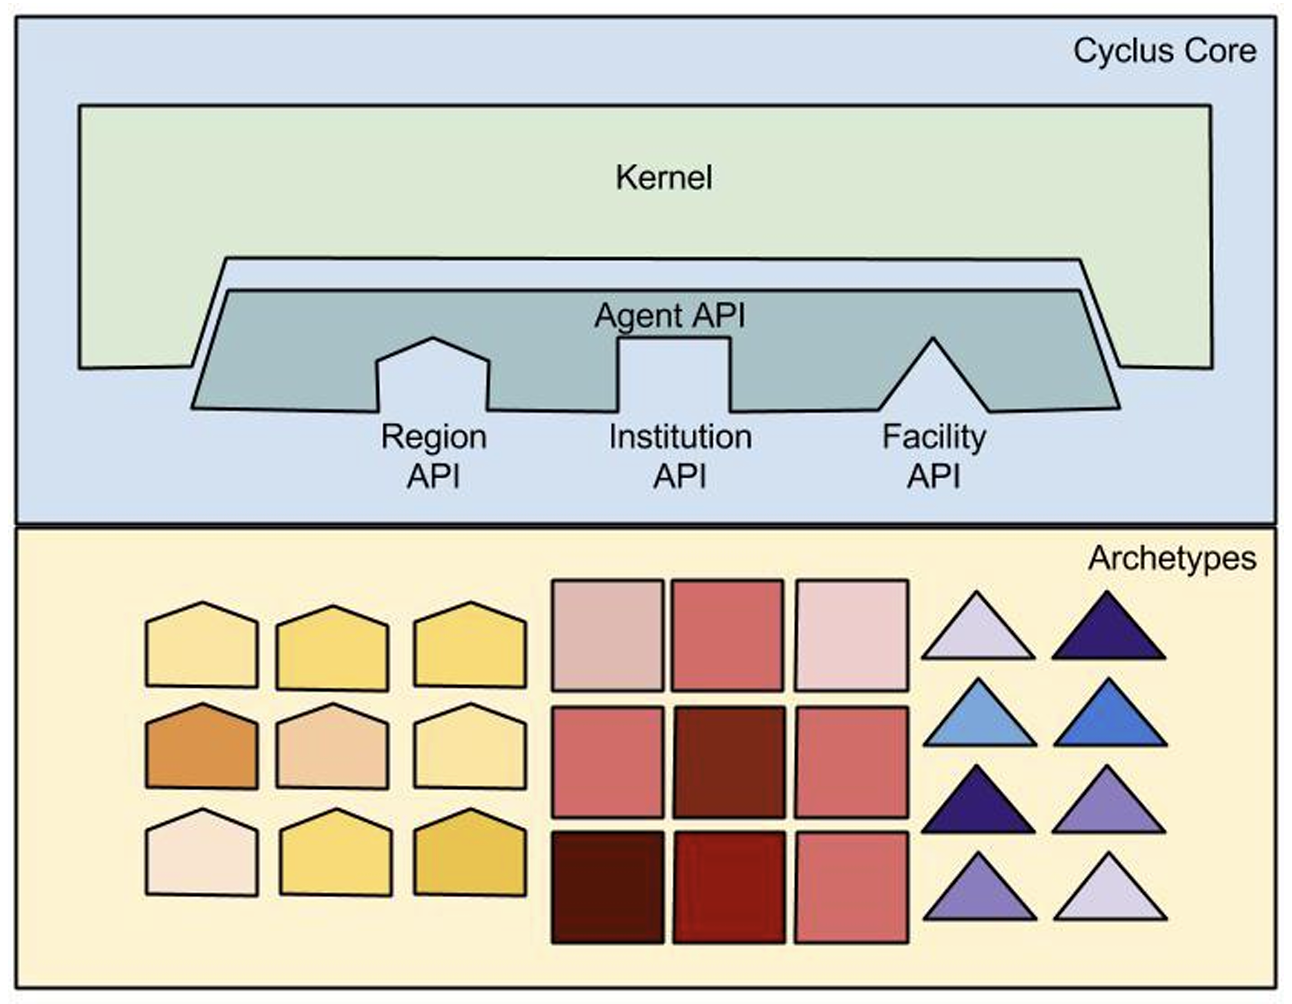
\includegraphics[width=0.75\textwidth]
        {figures/Cyclus.png}
    \caption{The \Cyclus simulation architecture separates the core kernel
    from dynamically loaded region, institution, and facility archetypes
    through the Agent \gls{API}. Figure reproduced from \cite{huff_fundamental_2016}.}
    \label{fig:cyclus-architecture}
\end{figure}


\subsection{Materials and Decay}
\label{subsec:cyclus-materials-decay}


Resources exchanged in \Cyclus are represented as discrete objects. The two
primary resource types are \emph{materials} and \emph{products}. A material
resource has an associated quantity and isotopic composition, whereas a
product represents a non-nuclear resource whose quality may be described
without a nuclide vector. Nuclear fuel cycle simulations therefore generally
use material resources to represent fresh fuel, spent nuclear fuel, separated
actinides, and radioactive waste \cite{huff_fundamental_2016}.

A \Cyclus material object contains a total mass and a \emph{Composition}
object. The composition stores the relative abundance of the nuclides present
in the material and is treated independently from the material quantity.
This separation allows multiple material objects to reference the same
composition and permits operations such as splitting, combining, and
transmuting material while preserving mass accounting. Materials may also
be stored in facility inventories and exchanged between agents through the
resource exchange system.

Radioactive decay can be applied directly to material resources within
\Cyclus. When a material is decayed over a specified time interval, its
nuclide vector is updated according to the radioactive decay chains available
to the framework. The decay calculation uses nuclear data supplied through
PyNE \cite{scopatzPyNEPythonNuclear2012}, which is an open-source nuclear engineering toolkit
that supplies the nuclear data including half-lives, decay constants, branching relationships, and
daughter products. The total quantity of a material remains associated with
the resource while its isotopic composition changes with time
\cite{huff_fundamental_2016}.

Decay in the simulations developed for this work is handled at the
simulation level through the \Cyclus control block, with decay set to
\texttt{lazy}. Under this setting the kernel decays a material's composition
on demand rather than at every time step, computing the decayed nuclide
vector when a composition is next inspected and caching the result for reuse
\cite{huff_fundamental_2016}. This choice retains the physical effect of
radioactive decay over the multi-decade simulation horizon while avoiding
the cost of decaying every inventory at every step. Decay is significant
over this horizon: the roughly 14-year half-life of \ce{^{241}Pu}, for
example, produces appreciable ingrowth of \ce{^{241}Am} across a
thirty-year run, altering the minor actinide vector that the inventory and
accelerator-driven system models are designed to track.


\subsection{The Dynamic Resource Exchange}
\label{subsec:cyclus-dre}

Transactions among \Cyclus facilities are coordinated through the \gls{DRE}. The \gls{DRE} provides a general
mechanism through which independently developed archetypes can exchange
resources without requiring direct knowledge of one another's internal
implementation. Facilities communicate their demand and supply to the
framework, and the exchange system determines a feasible set of transactions
for each time step \cite{huff_fundamental_2016}.

The exchange begins when consuming facilities generate requests for
resources. A request identifies a desired commodity, quantity, and, when
relevant, a target material composition or other resource quality. Supplying
facilities evaluate these requests and generate bids describing the resources
they are able to provide. A bid links a particular offered resource to a
request and may provide all or only part of the requested quantity\cite{gidden_agent-based_2015}.

Facilities may also assign preferences to possible trading partners or
resources. Preferences allow a requester to rank otherwise feasible bids,
for example by favoring a particular supplier, fuel composition, or material
characteristic. In addition, suppliers and requesters may impose constraints
such as production capacity, inventory availability, throughput, or minimum
and maximum transaction quantities. These constraints define which
combinations of trades are physically or operationally feasible.

The requests, bids, preferences, and constraints form a resource assignment
problem. \Cyclus formulates this assignment as an optimization problem, solvable in
either a linear or a mixed-integer form, and the \gls{DRE} solves it to select a
set of transactions that satisfies the applicable constraints while favoring
higher preference trades \cite{gidden_agent-based_2015}.
After the solution is determined, the participating facilities execute the
selected transactions and update their inventories. This process is repeated
at each simulation time step, allowing supply and demand relationships to
change dynamically as facilities are deployed, retired, depleted, or otherwise
alter their behavior.

By separating exchange coordination from facility specific behavior, the \gls{DRE}
allows archetypes to be developed and combined modularly. A storage facility,
reactor, separations plant, or repository can participate in the same exchange
system as long as it implements the appropriate request, bidding, and trade
interfaces. This separation is particularly important for this work because
the inventory and accelerator-driven system models must interact with both
existing and newly developed fuel cycle facilities.

\subsection{Extensions Developed in This Work}
\label{subsec:cyclus-extensions}

This work extends the \Cyclus ecosystem and its \texttt{cycamore} archetype library
\cite{carlsen_cycamore_2014} with two facility archetypes developed
within the \texttt{einstein} archetype library. The \texttt{us\_inventory}
facility represents the U.S. spent nuclear fuel inventory at assembly
resolution, reading isotopic compositions and assembly metadata from the
\gls{STANDARDS}~5.0.1 dataset\cite{peterson_unf-st&dards_2017,peterson_additional_2017}
and supplying material according to user-selected inventory selection policies.
The \texttt{ads} facility represents an accelerator-driven subcritical burner, transforming a
loaded core composition using a library of precomputed Serpent depletion
cases. Both archetypes participate in the resource exchange described above:
\texttt{us\_inventory} as a supplier whose selection policies determine which
assemblies it offers against a given request, and \texttt{ads} as a requester
whose feed preferences rank inventory and separations output. Their design,
implementation, and the four simulation scenarios in which they are exercised
are described in Chapter~\ref{ch:methodology}.


%%%%%%%%%%%%%%%%%%%%%%%%%%%%%%%%%%%%%%%%%%%%%%%%%%%%%%%%%%%%%%%%%%%%%%%%%%%%%%%%%%%%%%%%%%%%%%%%%%%%%%%%%%%%%%%%%%%%%%%%%%%%%%%%%%
%%%%%%%%%%%%%%%%%%%%%%%%%%%%%%%%%%%%%%%%%%%%%%%%%%%%%%%%%%%%%%%%%%%%%%%%%%%%%%%%%%%%%%%%%%%%%%%%%%%%%%%%%%%%%%%%%%%%%%%%%%%%%%%%%%%
%%%%%%%%%%%%%%%%%%%%%%%%%%%%%%%%%%%%%%%%%%%%%%%%%%%%%%%%%%%%%%%%%%%%%%%%%%%%%%%%%%%%%%%%%%%%%%%%%%%%%%%%%%%%%%%%%%%%%%%%%%%%%%%%

\section{Accelerator-Driven Systems}
\label{sec:ads}

\glspl{ADS} combine a high-power particle accelerator
with a subcritical nuclear assembly. They have been proposed as dedicated
systems for the transmutation of plutonium, minor actinides, and selected
long-lived fission products recovered from spent nuclear fuel
\cite{iaea_ma_fuels_2009}.
The \gls{ADS} concept is particularly relevant to this work because it provides a
potential pathway for consuming materials that is rich in minor actinides that present
significant neutronic and safety challenges in critical reactors.

\subsection{System Components and Operation}
\label{subsec:ads-components}

An \gls{ADS} consists of three principal components: a high-energy proton
accelerator, a spallation target, and a subcritical multiplying core. The
accelerator produces a proton beam, often with an energy of several hundred
megaelectronvolts to approximately one gigaelectronvolt. The beam strikes a
heavy metal target, where high energy proton-nucleus interactions release
neutrons through the spallation process. These source neutrons enter the
surrounding subcritical core and induce fission reactions in the fuel
\cite{aitabderrahim_myrrha_2001,nea_ads_components_2010}.

The target must generate a sufficiently intense neutron source while
withstanding substantial beam heating, radiation damage, and mechanical
loading. Heavy elements are attractive target materials because they produce
relatively large numbers of neutrons when bombarded by high-energy protons.
Proposed \gls{ADS} targets include solid tungsten targets and liquid metal targets
based on lead or lead-bismuth eutectic. In some designs, a circulating
liquid metal target also contributes to heat removal
\cite{aitabderrahim_myrrha_2001,nea_ads_components_2010}.

The core is designed to remain subcritical, such that

\begin{equation}
    k_{\mathrm{eff}} < 1,
\end{equation}

where \(k_{\mathrm{eff}}\) is the effective neutron multiplication factor.
Unlike a critical reactor, the neutron population in an \gls{ADS} core cannot
sustain itself indefinitely without the external spallation source. Source
neutrons initiate fission reactions and are multiplied within the subcritical
core, allowing the thermal power produced by fission to exceed the power
delivered by the proton beam
\cite{eriksson_ads_safety_2004,nea_ads_components_2010}.

The accelerator therefore provides an additional mechanism for controlling
the fission power. When the beam is interrupted, the external source of
spallation neutrons is removed and the source-driven fission power decreases
rapidly. This behavior is sometimes described by stating that the beam acts
as an on-off switch for the fission chain. However, turning off the beam
does not eliminate radioactive decay heat. The fuel and structures continue
to generate heat after shutdown and require reliable residual heat removal
\cite{eriksson_ads_safety_2004}.

Figure~\ref{fig:ads-components} illustrates the relationship among the
accelerator, spallation target, and subcritical core.

\begin{figure}[htbp]
    \centering
    \begin{tikzpicture}[
        node distance=2.5cm and 2.7cm,
        component/.style={
            rectangle,
            rounded corners,
            draw=black,
            minimum width=3.1cm,
            minimum height=1.1cm,
            align=center
        },
        flow/.style={thick,->,>=stealth}
    ]

    \node[component] (accelerator)
        {High-energy proton\\accelerator};

    \node[component, right=of accelerator] (target)
        {Spallation\\target};

    \node[component, right=of target] (core)
        {Subcritical core\\\(k_{\mathrm{eff}} < 1\)};

    \node[component, below=of core] (heat)
        {Heat removal and\\power conversion};

    \draw[flow]
        (accelerator) --
        node[above]{proton beam}
        (target);

    \draw[flow]
        (target) --
        node[above]{source neutrons}
        (core);

    \draw[flow]
        (core) --
        node[right]{thermal power}
        (heat);

    \end{tikzpicture}

    \caption{Principal components and energy flows of an
    accelerator-driven subcritical system. This original schematic is based
    on the \gls{ADS} descriptions presented in
    \cite{aitabderrahim_myrrha_2001,nea_ads_components_2010}.}
    \label{fig:ads-components}
\end{figure}

Accelerator-driven transmutation of used nuclear fuel received sustained
attention in the United States during the late 1990s and early 2000s, most
prominently through the \gls{ATW} program,
which developed system scenarios and integration roadmaps for dedicated
subcritical burners \cite{vantuyleRoadmapDevelopingATW2001}. Interest in the approach has
since reemerged in the context of managing the growing national
inventory.

\subsection{Minor Actinide Transmutation}
\label{subsec:ads-ma-transmutation}

The principal motivation for using \gls{ADS} technology for nuclear waste
management is its ability to accommodate fuels containing large fractions of
minor actinides. The minor actinides most commonly considered for
transmutation are neptunium, americium, and curium. These nuclides contribute
to the long-term radiotoxicity and decay heat of spent nuclear fuel. Their
separation and irradiation in a dedicated transmutation system could reduce
the quantity of long-lived transuranic material requiring disposal
\cite{iaea_ma_fuels_2009}.

Fast neutron spectra are generally preferred for minor actinide
transmutation because fission becomes more competitive with radiative
capture for many transuranic isotopes at higher neutron energies. A
fast spectrum system can therefore destroy minor actinides through fission
rather than merely converting them into heavier actinides
\cite{iaea_ma_fuels_2009}.

However, loading a critical fast reactor with a high concentration of minor
actinides introduces important safety and control challenges. Fuel rich in minor actinides
generally has a smaller effective delayed neutron fraction than
conventional uranium- or plutonium-bearing fuel. Although delayed neutrons
represent only a small fraction of the total fission neutron population, they
substantially slow the response of a critical reactor to reactivity changes.
A reduction in the effective delayed neutron fraction therefore causes the
reactor power to respond more rapidly to disturbances
\cite{eriksson_ads_safety_2004}.

Minor actinide loading may also reduce the magnitude of negative Doppler
reactivity feedback. In conventional reactor fuel, increasing fuel
temperature broadens neutron absorption resonances and generally introduces
negative reactivity. This prompt feedback opposes the temperature increase.
The magnitude of this effect can be weaker in minor actinide rich,
fast spectrum fuels because of their isotopic composition and the reduced
importance of resonance absorption in a fast spectrum
\cite{eriksson_ads_safety_2004,iaea_ma_fuels_2009}.

The combination of a reduced delayed neutron fraction and weaker negative
Doppler feedback makes a critical core with a high minor actinide content
more difficult to control. Critical fast reactor concepts may therefore limit
the amount of minor actinides loaded in the core or distribute them among
fuel containing larger quantities of uranium or plutonium\cite{eriksson_ads_safety_2004}.

Subcritical operation provides an alternative approach. Because the core
remains below criticality and relies on an external neutron source, an \gls{ADS}
can accommodate fuel compositions that would be difficult to use at high
concentrations in a critical reactor. Subcriticality provides additional
margin against prompt criticality and separates, to some extent, the control
of the neutron source from the inherent reactivity of the fuel
\cite{eriksson_ads_safety_2004}.

Subcriticality does not eliminate the need to evaluate reactivity accidents,
cooling failures, material behavior, or decay heat removal. Nevertheless, it
relaxes an important neutronic constraint on the amount of minor actinides
that can be loaded into a dedicated transmutation system. This capability is
the central reason that \gls{ADS} technology is relevant to this thesis. The
purpose of the modeled fuel cycle is to connect separated material from the
U.S. spent nuclear fuel inventory with systems capable of consuming
minor actinider streams that may not be suitable for concentrated use in
critical reactors.

\subsection{Target and Coolant Options}
\label{subsec:ads-target-coolant}

\gls{ADS} concepts differ in their target materials, coolants, fuel forms, neutron
spectra, and power levels. Lead and lead-bismuth eutectic are among the
most frequently proposed heavy liquid metals because their large atomic
masses support spallation neutron production and their high boiling
temperatures permit low pressure primary systems
\cite{aitabderrahim_myrrha_2001,nea_ads_components_2010}.

Lead-bismuth eutectics can have a substantially lower melting temperature than
pure lead, reducing some of the operational challenges associated with
coolant freezing. The most advanced current example is \gls{MYRRHA}, a lead-bismuth-cooled
subcritical system under development at the Belgian Nuclear Research Centre.
Its first phase, the \gls{MINERVA} proton accelerator and target facility, began
construction in 2024 \cite{dordaImplementationStatusMyrrha2024}, making \gls{MYRRHA} the closest
existing demonstration of the accelerator driven concept.
However, neutron activation of bismuth produces
polonium-210, which creates radiological and maintenance concerns. Both
lead and lead-bismuth can also cause corrosion or erosion of structural
materials. Their use therefore requires careful control of coolant chemistry,
oxygen concentration, temperature, and flow conditions
\cite{nea_ads_components_2010}.

Pure lead avoids the production of polonium associated with bismuth but has
a higher melting temperature. This increases the importance of freeze
prevention during startup, shutdown, and off-normal operation. Despite this
challenge, lead has been proposed both as a coolant and as a carrier medium
for mobile fuel \gls{ADS} concepts\cite{nea_ads_components_2010,gohar_ads_2021}.

The \gls{ADS} concept that provides the initial technical basis for the \gls{EINSTEIN}
project was developed to transmute material derived from the U.S. spent
nuclear fuel inventory. The proposed system uses a high energy proton
accelerator, a spallation neutron source, and a lead-based subcritical system.
The fuel concept contains plutonium and minor actinides in a mobile
lead-based medium, permitting continuous or periodic processing of the fuel
inventory \cite{gohar_ads_2021}.

Gas cooled \gls{ADS} concepts have also been investigated. Helium is chemically
inert and avoids many of the corrosion and activation issues associated with
heavy liquid metals. However, its low density and volumetric heat capacity
require high pressure operation and significant pumping power. The coolant
and target selection therefore influences neutron production, material
compatibility, plant efficiency, operating pressure, safety behavior, and
the design of the primary heat removal system
\cite{nea_ads_components_2010}.

\subsection{Technical and Economic Limitations}
\label{subsec:ads-limitations}

Despite their potential advantages for transmutation, \gls{ADS} facilities face
substantial technical and economic challenges. Accelerator availability is
one of the most important engineering concerns. A sudden beam interruption
causes a rapid decrease in fission power and temperature. Restoration of the
beam causes the power and temperature to increase again. Repeated beam
interruptions can therefore impose cyclic thermal loads on the fuel,
spallation target, coolant systems, and structural components
\cite{nea_beam_interruptions_2004}.

The \gls{OECD} Nuclear Energy Agency beam interruption benchmark specifically
examined the temperature transients caused by beam trips in a
lead-bismuth-cooled, subcritical system. The study identified thermal
fatigue of structural components as an important consequence of repeated
beam interruptions \cite{nea_beam_interruptions_2004}. More recent analysis
of the China Initiative Accelerator Driven System has also evaluated fuel
cladding fatigue under repeated beam trip transients
\cite{wang_beam_trips_2024}.

Producing a continuous, high-current proton beam with the availability
required for a power producing nuclear system is more demanding than
operating an accelerator intended for intermittent research use.
Fault-tolerant accelerator designs, redundant components, and rapid recovery
procedures may reduce the number and duration of beam interruptions, but
these features add complexity and cost
\cite{nea_ads_components_2010}.

The spallation target presents additional engineering challenges. It must
tolerate concentrated beam heating, radiation damage, gas production,
thermal stresses, and interactions with the coolant. Target replacement,
inspection, and maintenance must also be performed in a highly radioactive
environment \cite{nea_ads_components_2010}.

\gls{ADS} deployment additionally requires supporting fuel cycle infrastructure.
Spent nuclear fuel must first be processed to recover the actinides intended
for transmutation. The resulting material rich in minor actinides must then be
fabricated into fuel or introduced into an appropriate mobile fuel medium.
After irradiation, the material may require repeated separation and recycle
to achieve substantial actinide destruction. These activities introduce
material losses, secondary waste streams, safeguards requirements, worker
exposure, and additional facilities\cite{iaea_ma_fuels_2009}.

An \gls{ADS} also combines the capital cost and regulatory requirements of a
nuclear reactor facility with those of a high-power accelerator. Furthermore,
the accelerator consumes a portion of the electricity generated by the
system. Comparative \gls{OECD}/\gls{NEA} studies have therefore emphasized that the
potential transmutation benefits of \gls{ADS} technology must be evaluated
alongside its fuel cycle requirements, technical complexity, research and
development needs, and economic performance\cite{eriksson_ads_safety_2004}.

These limitations make a system level fuel cycle analysis necessary. The
performance of an \gls{ADS} cannot be judged solely from the rate of transmutation
inside its core. A complete assessment must also consider the availability
and composition of feed material, separations capacity, facility deployment,
accelerator and reactor throughput, recycle requirements, and the production
of secondary waste streams. These interactions motivate the \Cyclus
simulation models developed in this work.


%%%%%%%%%%%%%%%%%%%%%%%%%%%%%%%%%%%%%%%%%%%%%%%%%%%%%%%%%%%%%%%%%%%%%%%%%%%%%%%%%%%%%%%%%%%%%%%%%%%%%%%%%%%%%%%%%%%%%%%%%%%%%%%%%%
%%%%%%%%%%%%%%%%%%%%%%%%%%%%%%%%%%%%%%%%%%%%%%%%%%%%%%%%%%%%%%%%%%%%%%%%%%%%%%%%%%%%%%%%%%%%%%%%%%%%%%%%%%%%%%%%%%%%%%%%%%%%%%%%%%%
%%%%%%%%%%%%%%%%%%%%%%%%%%%%%%%%%%%%%%%%%%%%%%%%%%%%%%%%%%%%%%%%%%%%%%%%%%%%%%%%%%%%%%%%%%%%%%%%%%%%%%%%%%%%%%%%%%%%%%%%%%%%%%%%

\section{The EINSTEIN Program}
\label{sec:einstein}

The Enhanced Integrated Nuclear Systems for Transmutation and Efficient Isolation of Nuclides (\gls{EINSTEIN})
project is part of the \gls{ARPAE} Nuclear Energy Waste Transmutation Optimized Now (\gls{NEWTON}) program.
The \gls{NEWTON} program was established to support
technologies that enable the transmutation of used nuclear fuel and reduce
the burden placed on permanent waste disposal facilities
\cite{arpa_e_newton_2025}. The \gls{EINSTEIN} project is led by the University of Illinois Urbana-Champaign
\cite{arpa_e_einstein_2025}.

\gls{NEWTON} addresses the transmutation problem through three complementary
technical categories. Category A focuses on technologies for generating and
accelerating particle beams capable of initiating transmutation reactions.
Category B focuses on the design, fabrication, and processing of targets or
fuel forms containing the nuclides to be transmuted. Category C integrates
the technologies developed in Categories A and B through system level
modeling, life cycle analysis, techno-economic analysis, and databases of
materials and components
\cite{arpa_e_newton_2025,doe_categories}. \gls{UIUC} is a Category C and therefore
does not develop a single accelerator or transmutation target in isolation.
Instead, it provides a common framework for comparing candidate systems and
identifying the technical and economic conditions under which they could
contribute to management of the U.S. used nuclear fuel inventory.

Within the \gls{EINSTEIN} project, the term \acrshort{XDS} refers collectively
to subcritical transmutation systems sustained by an external neutron source.
Within this framing, \glspl{ADS} use an accelerator and spallation target to
produce the source neutrons, while \glspl{FDS} use neutrons generated by a
fusion source. The two classes may differ substantially in neutron energy,
source geometry, target and coolant materials, reliability constraints, and
technology readiness. Nevertheless, both couple an external neutron source to
a subcritical multiplying region and can therefore be represented within a
common fuel cycle and assessment framework. The initial \gls{EINSTEIN} analyses
include a high-energy, proton-driven, lead-cooled \gls{ADS} and a
\(14.1~\mathrm{MeV}\) fusion-neutron-driven, salt-cooled system
\cite{fang_einstein_2025}.

The central objective of \gls{EINSTEIN} is to develop a data-informed framework for
rapidly assessing \gls{XDS} technologies according to both their transmutation
performance and their financial implications. The project connects nuclear
data, neutronics, materials compatibility, fuel cycle behavior, and economic
performance rather than evaluating each component independently. The
official project description identifies the development of a comprehensive
life cycle analysis framework spanning the full transmutation process, from
the composition of the incoming used fuel stream through irradiation,
processing, and the resulting waste or product streams
\cite{arpa_e_einstein_2025}. Experimental and computational activities are
used to reduce uncertainties in neutron transport, material properties, and
component performance.

The \gls{UIUC} project team is organized around several interacting technical
areas as shown in Figure~\ref{fig:uiuc-einstein}. Nuclear data and diagnostics work identifies reactions whose
uncertainties significantly affect neutron multiplication and transmutation
predictions and develops experimental strategies to reduce those
uncertainties. Neutronics analysis provides source term, criticality,
depletion, and transmutation calculations for selected \gls{XDS} concepts.
Materials research evaluates corrosion, irradiation damage, thermophysical
properties, and the chemical behavior of lead coolants and molten salts.
Experimental work investigates the stability and solubility of representative
actinide surrogates and the compatibility of structural materials with the
candidate coolant and fuel media
\cite{fang_einstein_2025}.

\begin{figure}[htbp]
    \centering
    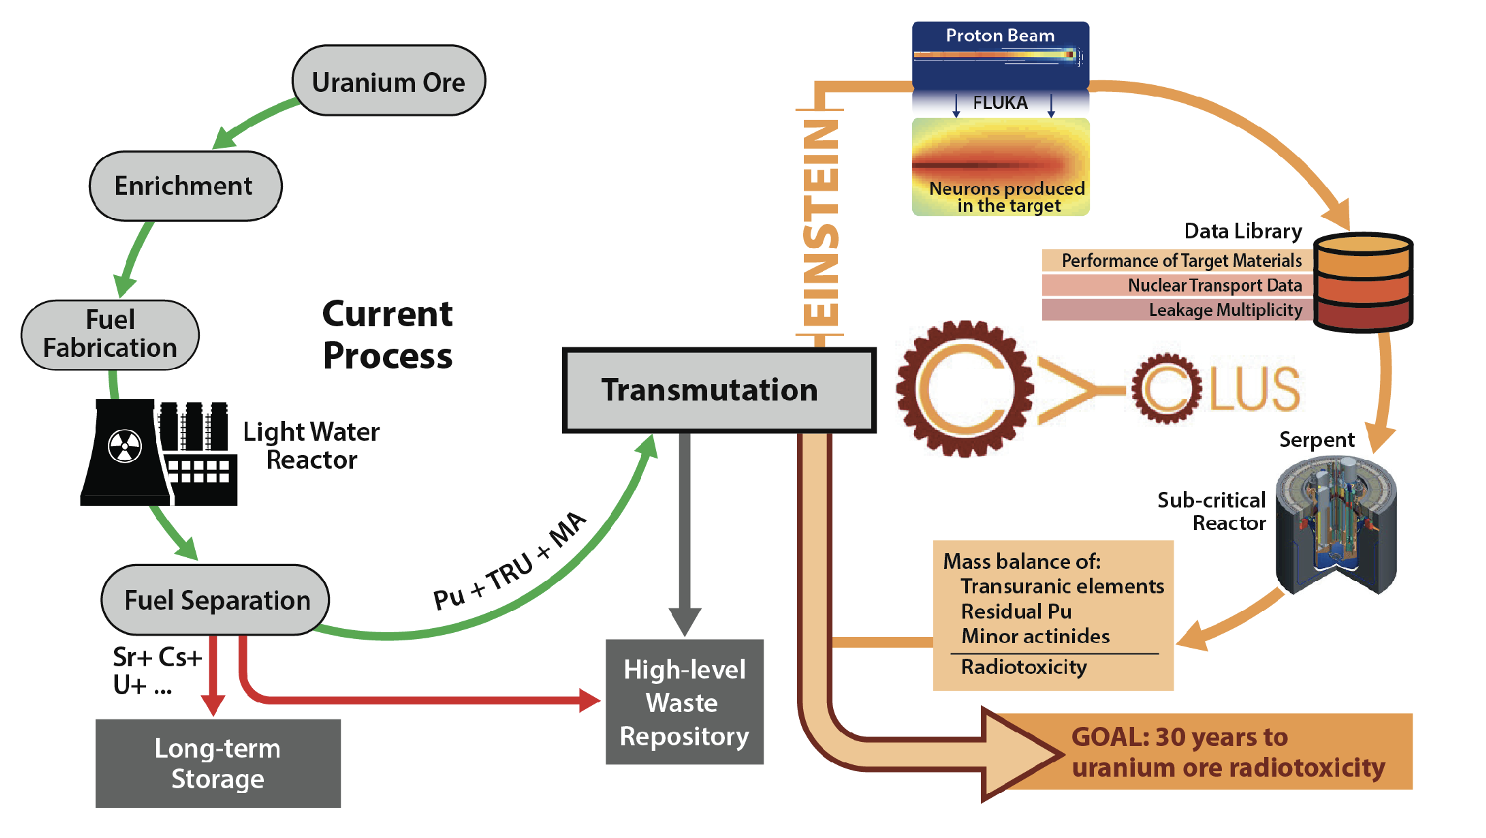
\includegraphics[width=\textwidth]
        {figures/EINSTEIN}
    \caption{Overview of the UIUC EINSTEIN project, which integrates FLUKA,
Serpent, nuclear data, materials, and \Cyclus fuel cycle analyses to evaluate
accelerator-driven transmutation of plutonium and minor actinides from used
nuclear fuel. The project aims to reduce the radiotoxicity of the remaining
waste to approximately that of natural uranium ore within 30 years. Figure reproduced from \cite{fang_einstein_2025}.}
    \label{fig:uiuc-einstein}
\end{figure}


These activities supply the inputs required for the fuel cycle and
techno-economic assessment. The fuel cycle portion of the project represents
the U.S. used nuclear fuel inventory, separations facilities, \gls{XDS} facilities,
recycle pathways, storage facilities, and waste streams in \Cyclus. The
inventory characterization begins with national spent fuel records and
age-corrected isotopic compositions, which are used to define realistic feed
streams for the modeled \gls{XDS} technologies. New \Cyclus archetypes are then
used to evaluate how the choice of feed material, facility throughput,
deployment schedule, separations capacity, and material selection policy
affects system level transmutation performance
\cite{fang_einstein_2025}.

The techno-economic analysis uses the outputs of the fuel cycle and
component models to examine capital costs, operating costs, potential
revenues, return on investment, and the sensitivity of economic conclusions
to uncertain design parameters. This coupling is important because a design
that performs well in a stand-alone neutronics calculation may still require
an impractical number of facilities, excessive separations capacity, costly
transportation, or unavailable supporting infrastructure. Conversely, a
concept with a lower per-facility transmutation rate may be more attractive
if it is easier to deploy, operate, and integrate with the existing nuclear
fuel cycle.

The work presented in this thesis lies primarily within the fuel cycle
modeling portion of \gls{EINSTEIN}. It develops the \texttt{us\_inventory} and
\texttt{ads} archetypes in the \texttt{einstein} library and uses them to
connect the characteristics of the national used fuel inventory with
candidate \gls{XDS} deployment scenarios. The resulting simulations provide
material flow, facility scaling, and inventory depletion information that can
be combined with the neutronics, materials, and economic analyses performed
elsewhere in the project. In this way, the thesis contributes the system level
link between the physical design of an \gls{XDS} and its potential effect on the
U.S. used nuclear fuel inventory.


%%%%%%%%%%%%%%%%%%%%%%%%%%%%%%%%%%%%%%%%%%%%%%%%%%%%%%%%%%%%%%%%%%%%%%%%%%%%%%%%%%%%%%%%%%%%%%%%%%%%%%%%%%%%%%%%%%%%%%%%%%%%%%%%%%
%%%%%%%%%%%%%%%%%%%%%%%%%%%%%%%%%%%%%%%%%%%%%%%%%%%%%%%%%%%%%%%%%%%%%%%%%%%%%%%%%%%%%%%%%%%%%%%%%%%%%%%%%%%%%%%%%%%%%%%%%%%%%%%%%%%
%%%%%%%%%%%%%%%%%%%%%%%%%%%%%%%%%%%%%%%%%%%%%%%%%%%%%%%%%%%%%%%%%%%%%%%%%%%%%%%%%%%%%%%%%%%%%%%%%%%%%%%%%%%%%%%%%%%%%%%%%%%%%%%%

\section{Prior Fuel Cycle Simulations of Transmutation Systems}
\label{sec:litrev}

Research on accelerator-driven transmutation has progressed through several
distinct stages. Early studies established the physics of coupling an intense
accelerator-produced neutron source to a subcritical multiplying medium.
Subsequent programs developed and tested individual enabling technologies,
including high current accelerators, liquid metal spallation targets,
subcriticality monitoring methods, minor actinide fuels, and lead or
lead-bismuth coolant systems. More recent studies have examined how dedicated
transmutation facilities could be incorporated into regional or national
nuclear fuel cycles.

These bodies of work do not all address the same modeling question. Reactor
physics studies generally evaluate neutron multiplication, power
distributions, safety coefficients, and nuclide destruction within one core.
Technology demonstrators test particular components or operating procedures.
Fuel cycle scenario studies instead examine the deployment of many reactors
and supporting facilities over several decades, tracking quantities such as
plutonium and minor actinide inventories, separations requirements, fuel
fabrication capacity, and waste production. The present work belongs primarily
to the third category, but its facility models are informed by the first two.

\subsection{European Demonstrator Programs}
\label{subsec:european-ads-programs}

Europe has sustained the most continuous multinational program of \gls{ADS}
research. Its development pathway has included conceptual system studies,
critical and subcritical experiments, a megawatt class liquid metal
spallation target experiment, and the staged development of the \gls{MYRRHA}
research facility. These programs have demonstrated important elements of an
\gls{ADS}, although no European facility has yet operated as a high power,
minor actinide burning \gls{ADS}.

One influential early European concept was Carlo Rubbia's
Energy Amplifier. The Energy Amplifier combined a high-energy proton
accelerator, a heavy metal spallation target, and a subcritical fast spectrum
blanket. Early versions emphasized energy production from thorium, while later
analyses also considered waste transmutation and fast spectrum operation
\cite{rubbia_conceptual_1995}. The importance of this work was not that
it produced a directly deployable fuel cycle design, but that it articulated
a complete accelerator target blanket system and stimulated coordinated
European research on spallation targets, lead-based coolants, subcritical
reactor physics, and partitioning and transmutation.

European research was subsequently coordinated through programs including
EUROTRANS, which investigated an experimental \gls{ADS} and the European Facility
for Industrial Transmutation \gls{EFIT}. \gls{EFIT} was conceived as a lead-cooled,
fast spectrum minor actinide burner rather than as a general-purpose power
reactor. Its design studies addressed accelerator requirements, target
integration, subcritical core design, dedicated minor actinide fuel, and the
supporting closed fuel cycle. In the ``double-strata'' strategy commonly
associated with these studies, conventional critical reactors would manage
most uranium and plutonium recycling, while a smaller fleet of dedicated \gls{ADS}
facilities would receive and destroy concentrated minor actinides\cite{nea_regional_scenarios_2009}.

The \gls{EFIT} studies are particularly relevant to fuel cycle analysis because
they treated an \gls{ADS} not as an isolated core but as one component of a broader
fleet. Regional scenario calculations examined the number of \gls{ADS} facilities
required to stabilize or reduce minor actinide inventories and estimated the
associated separations and fuelfabrication capacities. These analyses
demonstrated that transmutation performance depends not only on the
destruction rate of one \gls{ADS}, but also on cooling delays, reprocessing losses,
fuel fabrication throughput, deployment dates, and the availability of
separated feed material \cite{nea_regional_scenarios_2009}.

The principal European engineering demonstrator is \gls{MYRRHA} developed
by \gls{SCKCEN} in Belgium. \gls{MYRRHA} is designed as a lead-bismuth eutectic cooled,
fast spectrum research system capable of subcritical accelerator driven
operation and, in the broader design concept, critical operation. Its purposes
include demonstrating \gls{ADS} technology, conducting fuels and materials
irradiations, supporting radioisotope production, and providing experimental
data relevant to minor actinide transmutation
\cite{aitabderrahim_myrrha_2001,dordaImplementationStatusMyrrha2024}.

\gls{MYRRHA} is being implemented in phases. The first phase, \gls{MINERVA}, comprises
the lower-energy portion of the proton accelerator and associated target
stations. Construction of this phase began in 2024. The later phases would
extend the accelerator and couple it to the subcritical reactor. \gls{MYRRHA}
therefore represents the most advanced European program directed toward a
power scalable \gls{ADS}, but it should not yet be described as an operating
accelerator-driven reactor \cite{dordaImplementationStatusMyrrha2024}.

Several predecessor experiments were developed to reduce the technical risk
of \gls{MYRRHA}. The \gls{GUINEVERE} project coupled the \gls{GENEPI-3C} deuteron accelerator
to the \gls{VENUS-F} fast lead critical and subcritical assembly at \gls{SCKCEN}.
\gls{GUINEVERE} was designed principally to investigate reactor physics questions,
including the determination and online monitoring of subcriticality,
source jerk and beam interruption methods, core loading procedures, and the
transition between critical and subcritical configurations
\cite{billebaud_guinevere_2009,uyttenhove_experimental_2011,
marie_reactivity_2019}. It was a low-power experimental facility rather than
a fuel burning demonstrator, but it provided evidence that an accelerator
could be coupled to a fast subcritical assembly and that the system's
reactivity could be measured using realistic source operation modes.

A separate enabling technology experiment was the MEGAwatt Pilot Experiment,
or \gls{MEGAPIE}, operated at the Swiss spallation neutron source \gls{SINQ} in 2006.
\gls{MEGAPIE} exposed a circulating lead-bismuth target to a continuous
\(590~\mathrm{MeV}\) proton beam at approximately \(0.77~\mathrm{MW}\).
It was the first liquid metal spallation target operated in the megawatt beam
regime and supplied experimental data on neutron production, heat removal,
liquid metal operation, activation products, structural behavior, and
post-irradiation examination
\cite{bauer_megapie_2001,wagner_megapie_2008,
panebianco_neutronic_2007}. \gls{MEGAPIE} did not include a multiplying reactor core,
so it did not demonstrate an integrated \gls{ADS}. Its importance was instead the
validation of one of the most demanding \gls{ADS} components under an irradiation
environment approaching that required for a full-scale system.

France contributed to these European programs through \gls{CEA}, \gls{CNRS}, and other
institutions, as well as through national fuel cycle scenario studies. \gls{CEA}
developed the \gls{COSI} simulation code to model reactor fleets and associated
fuel cycle facilities over long time horizons. \gls{COSI} studies examined
transitions from light water reactors to sodium cooled fast reactors and
compared homogeneous, heterogeneous, and dedicated minor actinide
transmutation strategies
\cite{coquelet_pascal_cosi6_2015}.Other French and European studies compared
\gls{ADS}-based transmutation with minor actinide burning in critical fast reactors,
including differences in fuel cycle cost, inventory reduction, and supporting
facility requirements \cite{chabert_technical_2013,cross_check_2016}.

Taken together, the European programs established a progression from
component experiments to integrated demonstrator design and fleet-level
scenario analysis. \gls{GUINEVERE} addressed source coupling and subcriticality
monitoring, \gls{MEGAPIE} addressed a high power liquid metal target, \gls{EFIT} provided
a reference industrial transmuter design, and \gls{MYRRHA} seeks to integrate many
of these capabilities into a research facility. Their scenario studies also
showed that the viability of \gls{ADS} deployment cannot be inferred from
single core transmutation efficiency alone.

\subsection{United States Transmutation Programs, 1990s--2000s}
\label{subsec:us-transmutation-programs}

Modern U.S. accelerator-driven transmutation work grew partly from studies at
Los Alamos National Laboratory in the late 1980s and early 1990s. Bowman
et al.\ proposed coupling an intense accelerator-produced neutron source to a
subcritical multiplying and transmuting medium. The concept considered the
destruction of transuranic elements and selected long-lived fission products,
together with energy production from fertile material
\cite{bowman_nuclear_1992}. This work helped establish the
technical foundation for the (\gls{ATW})
program.

\gls{ATW} was developed during the 1990s as a system for treating commercial spent
nuclear fuel using partitioning, accelerator-driven transmutation, and
repeated recycle. A reference \gls{ATW} complex included front-end separations,
minor actinide and plutonium fuel preparation, one or more accelerator-driven
subcritical burners, recycle separations, and waste conditioning. The U.S.
Department of Energy submitted a development roadmap to Congress in 1999,
identifying required research in accelerators, spallation targets, separations,
fuels, materials, reactor physics, safety, and systems analysis
\cite{vantuyleRoadmapDevelopingATW2001,bellerUSAcceleratorTransmutation2001}.

The roadmap treated \gls{ATW} explicitly as a fuel cycle system rather than merely
as a reactor. This was important because repeated recycle is required to
achieve high actinide destruction. No irradiation cycle destroys every atom
fed to the system: some actinides remain in the discharged fuel, some are
converted into other actinides, and small fractions are lost during chemical
processing and fabrication. Consequently, the overall reduction in waste
burden depends on the efficiency and capacity of the complete recycle loop.

The follow-on \gls{AAA} program broadened the
scope of the U.S. effort to include waste transmutation, energy applications,
and enabling accelerator technologies. Program planning documents considered
the reliability of high power proton accelerators, liquid metal and solid
targets, subcritical blanket configurations, separations based on aqueous and
pyrochemical methods, and fabrication of fuels containing high fractions of
transuranic elements. Much of this work
remained at the level of design studies, laboratory research, and component
development. No integrated U.S. \gls{ATW} or \gls{AAA} engineering demonstrator was
constructed.

Systems studies performed for \gls{ATW} and related programs compared combinations
of light water reactors, critical fast reactors, and accelerator-driven
systems. These studies investigated questions such as whether plutonium
should first be recycled in light water reactors, whether \gls{ADS} facilities
should consume all transuranics or only minor actinides, and how many recycle
passes would be required. Their results repeatedly showed that conclusions
were sensitive to separations efficiency, fuel cooling time, accelerator
availability, support ratio, and the assumed growth or decline of nuclear
power \cite{vantuyleRoadmapDevelopingATW2001,bellerUSAcceleratorTransmutation2001}.


After the large \gls{ATW} and \gls{AAA} programs ended, U.S. \gls{ADS} work continued through
more focused reactor physics, materials, target, and systems studies. A recent
and particularly relevant example is the Argonne National Laboratory concept
reported by Gohar, Cao, and Kraus. Their design was developed specifically
to consume plutonium and minor actinides derived from the U.S. spent nuclear
fuel inventory. It employs a \(1~\mathrm{GeV}\) proton beam, a lead-based
spallation target, and a subcritical fast blanket with mobile fuel containing
plutonium and minor actinides
\cite{gohar_ads_2021}.

Gohar et al.\ used Monte Carlo transport and depletion calculations to examine
several blanket compositions and estimate the actinide consumption achievable
over decades of full-power operation. The study concluded that a small fleet
of large \gls{ADS} units could consume the minor actinide inventory assumed in its
analysis. However, its scope was a set of reference \gls{ADS} designs and their
depletion performance. It did not dynamically model the  level U.S.
inventory, site to site material movement, separations deployment,
facility construction schedules, or competition among facilities for
particular spent fuel resources. Thus, it provides the principal reactor
design basis for the \gls{ADS} model in this thesis, but not the system level model
needed to determine how that design would be supplied and deployed.

\subsection{Ongoing Construction: CiADS}
\label{subsec:ciads}

China began a national \gls{ADS} development program through the Chinese Academy
of Sciences in 2011. Early work included the
(\gls{CLEAR}) program and a series of lead-bismuth experimental loops, zero-power
facilities, and non-nuclear test systems. These activities supported the
development of coolant technology, structural materials, fuel assemblies,
components, and operating methods for a lead-cooled subcritical system
\cite{wu_design_2016}.

The China initiative Accelerator Driven System (CiADS), led by the Institute
of Modern Physics of the Chinese Academy of Sciences, is now under
construction in Huizhou. The integrated facility is designed to couple a
superconducting proton linear accelerator, a lead-bismuth spallation target,
and a lead-bismuth-cooled subcritical reactor. Published design studies
describe a first-stage reactor with a maximum thermal power of approximately
\(10~\mathrm{MW}\). The initial core uses oxide fuel and is intended primarily
to demonstrate the engineering feasibility, control, safety, and coupled
operation of the \gls{ADS} rather than to serve immediately as an industrial-scale
minor actinide burner
\cite{yin_power_2022,wang_transient_2023}.

CiADS is significant because it moves beyond isolated component tests toward
construction of an integrated accelerator target subcritical reactor
facility. Its research program addresses accelerator reliability, beam
transport, target behavior, lead-bismuth technology, reactor control,
thermal hydraulics, and protection systems. In the proposed operating
strategy, core power is controlled through the proton beam power because the
subcritical core does not contain a conventional critical reactor control
system for routine power regulation
\cite{yin_power_2022,li_control_2025}.

Dynamic and transient studies of CiADS have analyzed beam trips, beam
overpower, loss of flow, loss of heat sink, and station blackout conditions.
These calculations indicate substantial thermal margins for the low power
demonstrator while identifying longer term concerns such as lead-bismuth
corrosion, creep, and fatigue under repeated thermal cycling
\cite{wang_transient_2023}. The project therefore
provides an important test of whether the theoretically attractive
subcritical characteristics of \glspl{ADS} can be realized in a maintainable
engineering system.

CiADS should not be interpreted as a completed demonstration of a commercial
transmutation fuel cycle. The first stage system is much smaller than the
gigawatt thermal designs commonly assumed in industrial fuel cycle studies,
and its initial mission emphasizes technology demonstration. Nevertheless,
operational experience from CiADS could reduce major uncertainties presently
treated parametrically in systems models, including beam availability,
component lifetime, maintenance frequency, achievable capacity factor, and
the coupling between accelerator and reactor operation.

\subsection{Fuel Cycle Simulation Studies}
\label{subsec:ads-fuel-cycle-simulations}

The studies described above span a wide range of spatial and temporal
resolutions. Core design calculations may represent individual fuel pins and
detailed nuclide vectors but usually consider only one reactor and a limited
number of irradiation cycles. Fuel cycle simulators generally model decades
of fleet evolution, but they aggregate fuel into batches, reactor types, or
material streams. This trade-off between reactor detail and system breadth is
central to understanding the gap addressed by this thesis.

The \gls{OECD}/\gls{NEA} regional scenarios study extended this type of analysis to
groups of countries with different nuclear policies and fuel cycle
infrastructure. It used the \gls{EFIT} design as the reference \gls{ADS} and calculated
the number of transmuters and associated fuel cycle facilities required to
stabilize minor actinide inventories across a regional system
\cite{nea_regional_scenarios_2009}. This work showed that regional sharing of
specialized facilities could reduce duplication of expensive separations and
fabrication plants. However, its material representation was at the level of
national or regional inventory streams rather than individual discharged
assemblies.

France's \gls{COSI} code has been used extensively for dynamic scenario analysis.
\gls{COSI} represents reactor fleets, fuel fabrication, irradiation, cooling,
reprocessing, storage, and waste production over time. Applications have
included transitions from the existing French light water reactor fleet to
sodium-cooled fast reactors, along with comparisons of minor actinide
management options
\cite{coquelet_pascal_cosi6_2015}. These studies are highly detailed in their
treatment of fleet evolution and industrial fuel cycle capacity, but they
generally use reactor and fuel batches characterized by representative
compositions rather than a geospatially explicit assembly inventory.

European projects also compared the economic and material consequences of
minor actinide transmutation in critical fast reactors and \gls{ADS} facilities.
Chabert et al.\ compared no-transmutation, fast reactor, and \gls{ADS} options,
while Merino-Rodríguez et al.\ cross-checked economic and mass balance
calculations for scenarios involving dedicated \gls{ADS} burners
\cite{chabert_technical_2013,cross_check_2016}. These studies
demonstrated that \gls{ADS}-based strategies may achieve concentrated
minor actinide destruction but incur additional costs associated with the
accelerator, dedicated fuel fabrication, and supporting recycle facilities.

The Belgian \gls{ANICCA} code provides a more recent example directly related to
\gls{ADS} deployment. \gls{ANICCA} is a dynamic nuclear fuel cycle simulator developed
to study Belgian fleet evolution and waste management. A published
verification and case study examined the effect of adding an \gls{ADS} to a Belgian
nuclear phase-out scenario. The model tracked fleet-level materials and showed
the potential reduction of minor actinide inventories, but it did not model
individual commercial fuel assemblies or source site specific selection
\cite{rodriguez_nuclear_2020}.

Other studies have focused on detailed depletion within an \gls{ADS} rather than
deployment of the surrounding fuel cycle. These calculations optimize core
geometry, fuel loading, neutron spectrum, or recycle strategy and report
nuclide-specific transmutation rates. They are essential for supplying
performance parameters to a system model, but they do not themselves answer
how quickly suitable material becomes available, where it is stored, which
assemblies are selected, or how infrastructure limits deployment
\cite{gohar_ads_2021}.

Across the literature reviewed here, system level \gls{ADS} studies generally use
one of three material representations. The first is an equilibrium mass flow
model, in which annual production and destruction rates are balanced without
explicitly simulating each facility. The second is a dynamic fleet model in
which reactor types and fuel cycle plants are deployed over time and exchange
aggregated batches. The third is a detailed core or depletion model in which
a single \gls{ADS} is simulated at high isotopic resolution but the external fuel
cycle is prescribed rather than dynamically represented.

These approaches have provided estimates of \gls{ADS} support ratios, required
fleet size, equilibrium actinide inventories, separations capacity, fuel cycle
cost, and repository benefits. They have not generally represented the
existing U.S. used fuel inventory as a set of discrete assemblies carrying
site, discharge date, burnup, enrichment, mass, and composition metadata. In
the literature reviewed for this thesis, no prior \gls{ADS} fuel cycle study was
identified that dynamically selected individual assemblies from the
site-resolved U.S. inventory and supplied them through separations to
parameterized \gls{ADS} facilities.

Table~\ref{tab:prior-ads-studies} summarizes the different resolutions and
technical scopes represented by the major programs and simulation studies
discussed above.

\begin{table}[htbp]
    \centering
    \caption{Prior accelerator-driven transmutation programs and studies
    addressed different levels of technology and fuel cycle resolution.
    Information summarized from
    \cite{dordaImplementationStatusMyrrha2024,billebaud_guinevere_2009,
    wagner_megapie_2008,gohar_ads_2021,
    wang_transient_2023,nea_regional_scenarios_2009,
    rodriguez_nuclear_2020}.}
    \label{tab:prior-ads-studies}

    \begin{tabularx}{\textwidth}{@{}p{2.0cm}p{2.3cm}Xp{2.5cm}@{}}
        \toprule
        \textbf{Program or study}
        & \textbf{Type}
        & \textbf{Principal scope}
        & \textbf{Material resolution} \\
        \midrule

        \gls{GUINEVERE}
        & Experimental facility
        & Accelerator coupling, fast subcritical physics, and online
          reactivity monitoring
        & Core configurations; no fuel cycle deployment \\

        \gls{MEGAPIE}
        & Component experiment
        & Megawatt-class liquid lead-bismuth spallation target
        & Target and neutron source behavior only \\

        \gls{MYRRHA}
        & Staged demonstrator
        & Accelerator, target, fast spectrum research reactor, fuels,
          materials, and \gls{ADS} operation
        & Core and irradiation experiments; supporting scenario studies \\

        \gls{EFIT} / European scenarios
        & Reference design and fleet studies
        & Dedicated minor actinide burning and regional deployment
        & Aggregated fuel batches and regional inventories \\

        \gls{ATW} / \gls{AAA}
        & U.S. program and system studies
        & Separations, recycle, accelerator, target, and subcritical burner
        & Process streams and representative fuels \\

        Gohar et al.
        & \gls{ADS} design and depletion study
        & Lead-based mobile fuel \gls{ADS} for the U.S. actinide inventory
        & Prescribed blanket compositions \\

        CiADS
        & Integrated demonstrator under construction
        & Coupled accelerator, spallation target, and low-power
          subcritical reactor
        & Detailed core and component models \\

        \gls{COSI} / \gls{ANICCA} studies
        & Dynamic fuel cycle simulation
        & Fleet transitions, facility capacities, inventories, and waste
        & Reactor fleets and aggregated fuel batches \\

        This work
        & Dynamic fuel cycle simulation
        & U.S. inventory selection, separations, \gls{ADS} deployment,
          throughput, and inventory evolution
        & Individual assemblies with associated metadata \\
        \bottomrule
    \end{tabularx}
\end{table}

That distinction is important for the U.S. case. The national inventory is
not an equilibrium material stream produced by a uniform reactor fleet. It is
a heterogeneous legacy inventory accumulated over several decades and stored
at geographically dispersed operating and shutdown sites. Assemblies differ
in age, burnup, enrichment, reactor type, remaining heavy metal mass, isotopic
composition, and storage location. A model that begins with a representative
average composition cannot evaluate how alternative inventory selection
policies change the material supplied to separations and transmutation
facilities.

The present work addresses this gap by combining an assembly resolved U.S.
inventory facility with dynamically deployed \gls{ADS} and supporting fuel cycle
facilities in \Cyclus. It does not replace detailed neutronics, depletion,
materials, or economic models. Instead, it provides the system layer through
which those models can be connected to the actual characteristics and
availability of U.S. used nuclear fuel. This representation permits analysis
of inventory selection policies, throughput limits, facility scaling,
deployment timing, material availability, and the evolution of the remaining
national inventory.


%%%%%%%%%%%%%%%%%%%%%%%%%%%%%%%%%%%%%%%%%%%%%%%%%%%%%%%%%%%%%%%%%%%%%%%%%%%%%%%%%%%%%%%%%%%%%%%%%%%%%%%%%%%%%%%%%%%%%%%%%%%%%%%%%%
%%%%%%%%%%%%%%%%%%%%%%%%%%%%%%%%%%%%%%%%%%%%%%%%%%%%%%%%%%%%%%%%%%%%%%%%%%%%%%%%%%%%%%%%%%%%%%%%%%%%%%%%%%%%%%%%%%%%%%%%%%%%%%%%%%%
%%%%%%%%%%%%%%%%%%%%%%%%%%%%%%%%%%%%%%%%%%%%%%%%%%%%%%%%%%%%%%%%%%%%%%%%%%%%%%%%%%%%%%%%%%%%%%%%%%%%%%%%%%%%%%%%%%%%%%%%%%%%%%%%

\section{Research Gap}
\label{sec:gap}

The literature reviewed in Section~\ref{sec:litrev} demonstrates substantial
progress in accelerator-driven transmutation, but the principal areas of
progress have remained separated. Reactor physics and engineering studies
have developed increasingly detailed representations of accelerators,
spallation targets, subcritical cores, fuels, coolants, and transmutation
performance. Fuel cycle studies have examined the deployment of reactors,
separations plants, fabrication facilities, and waste management
infrastructure over long periods. National spent fuel databases have also
developed sufficiently detailed records to characterize individual discharged
fuel assemblies. However, these capabilities have not generally been combined
in a single simulation. In the literature reviewed for this thesis, no
published study was identified that dynamically couples a real,
assembly resolved U.S. spent nuclear fuel inventory to an \gls{ADS} facility inside
a fuel cycle simulator and evaluates how the selection of particular
assemblies affects transmutation system deployment and the evolution of the
remaining national inventory.

European \gls{ADS} research has produced the most mature combination of
experimental facilities, component demonstrations, core calculations, and
regional fuel cycle studies. \gls{GUINEVERE} investigated accelerator coupling and
subcriticality monitoring, \gls{MEGAPIE} demonstrated a liquid metal spallation
target under a megawatt-class proton beam, and \gls{MYRRHA} has advanced the
engineering design and staged implementation of an integrated \gls{ADS} research
facility
\cite{aitabderrahim_myrrha_2001,billebaud_guinevere_2009,
uyttenhove_experimental_2011,wagner_megapie_2008,
dordaImplementationStatusMyrrha2024}. European fuel cycle tools have also
examined fleet transitions and minor actinide transmutation. For example,
\gls{COSI} has been used to evaluate French reactor and fuel cycle transitions,
while \gls{ANICCA} has modeled the introduction of an \gls{ADS} into a Belgian nuclear
phase-out scenario
\cite{coquelet_pascal_cosi6_2015,rodriguez_nuclear_2020}.
These studies provide detailed information about European reactor fleets,
fuel cycle infrastructure, and transmutation strategies, but their feed
materials are represented as reactor specific or scenario specific fuel
streams and batches. They do not begin with the discrete assembly records of
the existing U.S. inventory or evaluate alternative rules for selecting
particular U.S. assemblies for processing.

The U.S. Accelerator Transmutation of Waste and Advanced Accelerator
Applications programs addressed many policy relevant aspects of a complete
transmutation system. Their roadmaps and system studies considered
separations, repeated actinide recycle, fuel fabrication, accelerator
reliability, spallation target design, subcritical burners, and final waste
management
\cite{vantuyleRoadmapDevelopingATW2001,
bellerUSAcceleratorTransmutation2001}.
These efforts recognized that the performance of an \gls{ADS} could not be assessed
independently from the facilities that prepare, recycle, and manage its fuel.
Nevertheless, the principal \gls{ATW} and \gls{AAA} studies were conducted before the
development of current agent-based fuel cycle simulators and before the
availability of the present assembly level \gls{STANDARDS} database. Consequently,
their national inventory was represented through assumed aggregate material
streams, reference isotopic compositions, and projected production rates
rather than through the individual assemblies that constitute the existing
U.S. inventory.

More recent U.S. work has improved the physical basis of the \gls{ADS} itself.
Gohar, Cao, and Kraus developed a lead-based \gls{ADS} concept specifically for
consuming plutonium and minor actinides derived from U.S. spent nuclear fuel
and used detailed transport and depletion calculations to estimate actinide
consumption over the operating life of the system
\cite{gohar_ads_2021}. This study provides the initial \gls{ADS} design basis used
in the present work, but its treatment of the national inventory begins with
the total assumed masses of plutonium and minor actinides. It does not model
the discharged assemblies from which those materials would be recovered, the
order in which assemblies would be selected, or the time-dependent
interaction among inventory, separations, and \gls{ADS} facilities.

CiADS addresses a different part of the problem. Its published analyses
focus on the engineering behavior of an integrated accelerator, spallation
target, and low-power subcritical reactor. Studies have examined proton beam
control, reactor transients, beam trips, thermal margins, coolant behavior,
and structural fatigue
\cite{wu_design_2016,yin_power_2022,wang_transient_2023,
wang_beam_trips_2024}. This work is essential for demonstrating whether \gls{ADS}
technology can be operated reliably, but CiADS is an engineering
demonstrator rather than a simulation of national fuel cycle deployment. Its
analyses therefore do not address how a heterogeneous legacy inventory would
be selected, transported, separated, and allocated among multiple future
transmutation facilities.

Existing fuel cycle and inventory studies come closest to connecting these
areas. The \gls{STANDARDS}~5.0.1 Database contains detailed information
about the \gls{SNF} inventory in the U.S. with full isotopic composition.
Peterson et al.\ described the planned use of \gls{UDB} information in system models
such as \gls{NGSAM} and in fuel cycle transition analyses using \gls{ORION}
\cite{peterson_additional_2017}. Bae et al.\ subsequently trained a neural
network on \gls{UDB} depletion data and implemented the resulting model in
\Cyclus, enabling efficient prediction of spent fuel compositions for
reactor batches with varying burnup and enrichment
\cite{bae_deep_2020}. These studies established that realistic U.S. data can
improve fuel cycle simulation. The former described broader integration of
the database with system and fuel cycle tools, while the latter reproduced
\gls{UDB}-derived isotopic behavior without exposing or dynamically transacting
the underlying private assembly records. Neither work connected an active
assembly inventory to an \gls{ADS} burner or examined how the choice among
available assemblies changes the feed supplied to that burner.

The gap addressed in this thesis is therefore narrower than the absence of
either detailed \gls{ADS} models or detailed inventory data. The missing capability
is their integration at the system level. This work represents individual
U.S. spent fuel assemblies as selectable resources within an agent-based
fuel cycle simulation. Assembly records derived from \gls{STANDARDS}~5.0.1 retain
attributes relevant to material selection, including available heavy metal
mass, discharge date, burnup, initial enrichment, and isotopic composition
\cite{carter_banerjee_inventory_2024}. The
\texttt{us\_inventory} archetype supplies these resources through the
\Cyclus Dynamic Resource Exchange rather than first collapsing the national
inventory into a single average recipe.

The inventory model is coupled to an \gls{ADS} archetype whose material
transformation is based on precomputed Serpent depletion results. The
simulation can therefore evaluate multiple inventory selection policies,
including selection by availability, age, burnup, and enrichment, while
maintaining material accounting as assemblies are supplied and their
available masses are depleted. The results presented in
Chapters~\ref{ch:methodology}-\ref{ch:results} quantify how these policies
change the mass and characteristics of material supplied to the modeled
fuel cycle facilities and how they alter the composition of the inventory
remaining after transmutation.

This integration does not by itself constitute a complete recommendation for
U.S. waste policy. Questions involving facility siting, transportation
approval, safeguards, separations readiness, cost, financing, and repository
performance require additional models and institutional assumptions. Rather,
the contribution of this thesis is to provide a U.S.-specific material flow
foundation on which those analyses can be built. By connecting an
assembly resolved legacy inventory to an \gls{ADS} representation in \Cyclus, the
work enables transmutation scenarios to be evaluated using the actual
heterogeneity and availability of U.S. spent nuclear fuel instead of an
assumed national average feed.